\documentclass[aspectratio=169, 12pt]{beamer}

% --- NOTES SETUP ---
% Comment out for final submission (no speaker notes)
% \usepackage{pgfpages}
% \setbeameroption{show notes on second screen=right} % Shows notes on the right side

% Theme - Modern but compatible
\usetheme{Boadilla}
\usecolortheme{whale}
% Add some modern touches
\setbeamertemplate{navigation symbols}{}  % Remove navigation symbols
% Custom footline that respects [noframenumbering]
\setbeamertemplate{footline}{
  \leavevmode%
  \hbox{%
  \begin{beamercolorbox}[wd=\paperwidth,ht=2.25ex,dp=1ex,right]{date in head/foot}%
    \usebeamerfont{date in head/foot}\insertframenumber{} / \inserttotalframenumber\hspace*{2ex}
  \end{beamercolorbox}}%
  \vskip0pt%
}

% Packages
\usepackage{graphicx}
\usepackage{tikz}
\usepackage{booktabs}
\usepackage{amsmath}
\usepackage{fontawesome5}
\usepackage{colortbl}
\usepackage{tcolorbox}

% Load TikZ libraries
\usetikzlibrary{shadows, calc, shapes, positioning, shadows.blur, decorations.pathreplacing, fadings, backgrounds, fit}

% Better font rendering
\usepackage{lmodern}

% =================== CUSTOM COLOR PALETTE ===================
\definecolor{PrimaryBlue}{RGB}{0, 82, 155}        % Deep professional blue
\definecolor{AccentOrange}{RGB}{230, 97, 0}       % Warm accent
\definecolor{TheoreticalBlue}{RGB}{52, 152, 219}  % Lighter blue for theory
\definecolor{PracticalGreen}{RGB}{46, 204, 113}   % Fresh green for practice
\definecolor{BridgeTeal}{RGB}{22, 160, 133}       % Sophisticated teal
\definecolor{ShadowGray}{RGB}{189, 195, 199}      % Subtle shadows
\definecolor{BackgroundLight}{RGB}{250, 250, 250} % Off-white backgrounds

% Enhanced Beamer color customization
\setbeamercolor{structure}{fg=PrimaryBlue}
\setbeamercolor{frametitle}{bg=PrimaryBlue!8, fg=PrimaryBlue}
\setbeamercolor{block title}{bg=PrimaryBlue!15, fg=PrimaryBlue}
\setbeamercolor{block body}{bg=PrimaryBlue!5}
\setbeamercolor{block title example}{bg=PracticalGreen!20, fg=PracticalGreen!80!black}
\setbeamercolor{block body example}{bg=PracticalGreen!5}
\setbeamercolor{block title alerted}{bg=AccentOrange!20, fg=AccentOrange!80!black}
\setbeamercolor{block body alerted}{bg=AccentOrange!5}

% Modern bullet points
\setbeamertemplate{itemize items}[circle]
\setbeamertemplate{itemize item}{\small\textcolor{PrimaryBlue}{\textbullet}}
\setbeamertemplate{itemize subitem}{\tiny\textcolor{PrimaryBlue!70}{$\blacktriangleright$}}

% TikZ fade definitions
\tikzfading[name=fade out, inner color=transparent!0, outer color=transparent!100]

% Modern tcolorbox presets
\tcbset{
    modernbox/.style={
        colback=#1!5,
        colframe=#1!60,
        boxrule=1pt,
        arc=3pt,
        left=5pt,
        right=5pt,
        top=4pt,
        bottom=4pt,
        shadow={1mm}{-1mm}{0mm}{black!20}
    }
}

% Path to your images
\graphicspath{{./images/}}

% Meta
\title[Cognitive MRI of AI Conversations]{Cognitive MRI of AI Conversations:\\A Single-User Case Study}
\subtitle{Revealing the Hidden Topology of Thought}
\author{Alex Towell \and John Matta}
\institute[SIUE]{Southern Illinois University Edwardsville}
\date{}

\begin{document}

%---------------------------------------------------------
% 1. Title - ENHANCED
%---------------------------------------------------------
\begin{frame}[plain]
    % Background design elements
    \begin{tikzpicture}[remember picture, overlay]
        % Subtle gradient background
        \fill[PrimaryBlue!5] (current page.north west) rectangle (current page.south east);
        % Decorative accent bar at top
        \fill[PrimaryBlue] (current page.north west) rectangle ([yshift=-0.25cm]current page.north east);
        % Subtle accent at bottom
        \fill[ShadowGray, opacity=0.08] ([yshift=1.5cm]current page.south west) rectangle (current page.south east);
    \end{tikzpicture}

    \setlength{\columnsep}{18pt}
    \begin{columns}[T]
        \column{0.65\textwidth}
        \vspace{1cm}

        % Title with enhanced visual hierarchy
        {\fontsize{22}{26}\selectfont\textcolor{PrimaryBlue}{\textbf{Cognitive MRI of AI Conversations:}}}\\[0.25cm]
        {\fontsize{22}{26}\selectfont\textcolor{PrimaryBlue}{\textbf{A Single-User Case Study}}}\\[0.5cm]

        % Subtitle
        {\large\textcolor{black!70}{Revealing the Hidden Topology of Thought}}\\[0.9cm]

        % Authors
        {\large\textbf{Alex Towell} \quad \textbf{John Matta}}\\[0.25cm]
        {\normalsize\textit{Southern Illinois University Edwardsville}}\\[0.15cm]
        {\normalsize\texttt{\textcolor{PrimaryBlue}{\{atowell,jmatta\}@siue.edu}}}\\[1cm]

        % Repository link
        {\footnotesize\faGithub\ Code \& Data: \textcolor{PrimaryBlue}{\url{github.com/queelius/chatgpt-complex-net}}}

        \column{0.35\textwidth}
        \vspace{1.3cm}
        \centering
        % Logo with subtle shadow
        \begin{tikzpicture}
            \node[drop shadow={shadow xshift=0.08cm, shadow yshift=-0.08cm, opacity=0.25}]
                {\includegraphics[width=0.9\textwidth]{logo_cna2025_textblue.png}};
        \end{tikzpicture}
    \end{columns}

    \note{
        \textbf{Slide 1: Title (30s)}
        \begin{itemize}
            \item \textbf{Hook:} ``Good morning. We often think of our interactions with AI as just `chats'---fleeting lines of text. But what if we treated them as a dataset of \textit{thought}?''
            \item \textbf{Core Question:} ``Can we take the linear logs of a single user and reconstruct the `shape' of their knowledge?''
            \item \textbf{Analogy:} ``We call this a \textbf{Cognitive MRI}. Just as an MRI images the physical structure of the brain from magnetic signals, we are imaging the \textit{conceptual} structure of the mind from semantic signals.''
            \item \textbf{Bridge (5s):} ``But before we dive into one user's map, let's understand why this matters at a planetary scale.''
        \end{itemize}
    }
\end{frame}

%---------------------------------------------------------
% 2. NEW: Why Now? The Scale of the Opportunity
%---------------------------------------------------------
\begin{frame}{Why Now? The Scale of the Opportunity}
    \begin{columns}[T]
        % LEFT: Visual representation of scale
        \column{0.5\textwidth}
        \centering
        \vspace{0.3cm}

        \textbf{$\sim$1 Billion ChatGPT Users}

        \vspace{0.3cm}

        % TikZ: Enhanced globe with depth
        
\begin{tikzpicture}[scale=1.2]
            % Globe with layered effect for depth
            \foreach \r/\op in {1.52/0.05, 1.51/0.1, 1.50/0.2} {
                \draw[thick, PrimaryBlue!50, opacity=\op, line width=1.2pt] (0,0) circle (\r cm);
            }
            \draw[thick, PrimaryBlue!60, line width=1.5pt] (0,0) circle (1.5cm);

            % Equator and meridian
            \draw[thick, PrimaryBlue!50, line width=1pt] (0,0) ellipse (1.5cm and 0.5cm);
            \draw[thick, PrimaryBlue!50, line width=1pt] (-1.5,0) arc (180:360:1.5cm and 1.5cm);

            % Latitude lines for depth
            \draw[PrimaryBlue!30, line width=0.5pt] (0,0.75) ellipse (1.3cm and 0.3cm);
            \draw[PrimaryBlue!30, line width=0.5pt] (0,-0.75) ellipse (1.3cm and 0.3cm);

            % User icons with glow effect
            \foreach \angle/\radius in {30/1.2, 80/1.3, 130/1.1, 200/1.3, 260/1.2, 310/1.4} {
                \fill[PrimaryBlue!20, opacity=0.4] (\angle:\radius) circle (0.15cm);
                \node[PrimaryBlue!80, font=\small] at (\angle:\radius) {\faUser};
            }

            % Central emphasis with shadow
            \node[font=\large, text=PrimaryBlue, align=center,
                  drop shadow={shadow xshift=0.03cm, shadow yshift=-0.03cm, opacity=0.2}] at (0,-2.3) {
                \textbf{Global Scale}\\[0.1cm]
                \scriptsize Unprecedented access to\\[-0.05cm]
                \scriptsize cognitive processes
            };
        \end{tikzpicture}

        \column{0.5\textwidth}
        \vspace{0.2cm}

        \textbf{Chat logs capture something different:}

        \vspace{0.3cm}

        \begin{itemize}
            \setlength\itemsep{0.4em}
            \item \textbf{Citations} $\rightarrow$ papers (outputs)
            \item \textbf{Social networks} $\rightarrow$ connections
            \item \textbf{Chat logs} $\rightarrow$ \textcolor{PracticalGreen!80!black}{\textbf{the process}}
        \end{itemize}

        \vspace{0.4cm}

        \begin{block}{}
            \centering
            \small
            How ideas develop. The back-and-forth.\\[0.3em]
            \textit{Today: one case study.}
        \end{block}
    \end{columns}

    \note{
        \textbf{Slide 2: Scale \& Stakes (45s)}
        \begin{itemize}
            \item \textbf{Context:} ``Before we dive into methods, why does this matter?''
            \item \textbf{Scale:} ``ChatGPT has 1.7 billion users. Each one generating conversational traces of their thought process.''
            \item \textbf{Uniqueness:} ``Traditional datasets---citations, social networks---only capture the \textit{output}. They don't capture the iterative reasoning.''
            \item \textbf{Opportunity:} ``This is the first time in history we have access to the \textit{process} at global scale.''
            \item \textbf{Bridge to Methods:} ``Today we'll show a single-user case study. But the method generalizes. Imagine mapping the collective knowledge structure of entire research communities.''
        \end{itemize}
    }
\end{frame}

%---------------------------------------------------------
% 3. The Big Picture - EXTERNALIZED COGNITION
%---------------------------------------------------------
\begin{frame}{The Big Picture: Externalized Cognition}
    \begin{columns}[T]
        % --- LEFT COLUMN: The Narrative ---
        \column{0.55\textwidth}
        \small
        \textbf{AI conversations are not just chat logs.}

        \vspace{0.1cm}
        We view them through the lens of \textbf{Distributed Cognition}:
        \begin{itemize}
            \setlength\itemsep{0.1em}
            \item \textbf{Thinking Out Loud:} The user offloads cognitive load to the machine.
            \item \textbf{The Iterative Loop:} Ideas aren't just ``retrieved''; they are constructed through dialogue.
        \end{itemize}

        % CRITICAL FIX: Negative spacing to pull the block up
        \vspace{-0.3cm}

        \begin{alertblock}{The ``Cognitive Dark Matter''}
            \footnotesize
            Standard archives preserve the \emph{result} (the paper). \\
            LLM logs capture the \emph{process}---the false starts, synthesis, reasoning.
        \end{alertblock}

        % --- RIGHT COLUMN: The "Iceberg" Graphic ---
        \column{0.45\textwidth}
        \centering
        \begin{tikzpicture}[scale=0.95, transform shape]
            % --- WATERLINE with depth effect ---
            \fill[PrimaryBlue!5, opacity=0.4] (-2.5, 0) rectangle (2.5, -4);
            \draw[PrimaryBlue!50, line width=1.5pt] (-2.5, 0) -- (2.5, 0);
            \node[fill=white, text=PrimaryBlue!70, font=\scriptsize\bfseries,
                  rounded corners=2pt, inner sep=2pt] at (0,0) {Visibility Threshold};

            % --- TOP: THE ARTIFACT (The Paper) ---
            \node[anchor=south] at (0, 0.5) {
                \begin{tikzpicture}
                    % Paper shadow
                    \fill[ShadowGray!30, rounded corners=1pt] (0.08,-0.08) rectangle (1.28, 1.52);
                    % Paper Icon
                    \draw[fill=white, draw=gray!50, line width=0.8pt] (0,0) rectangle (1.2, 1.6);
                    % Folded corner effect
                    \fill[gray!15] (0.9,1.6) -- (1.2,1.6) -- (1.2,1.3) -- cycle;
                    \draw[gray!50, line width=0.5pt] (0.9,1.6) -- (0.9,1.3) -- (1.2,1.3);
                    % Text lines with varying opacity
                    \foreach \y/\op in {1.2/0.7, 1.0/0.6, 0.8/0.5, 0.6/0.4, 0.4/0.3} {
                        \draw[gray, opacity=\op, line width=1pt] (0.15, \y) -- (0.85, \y);
                    }
                    \node[font=\tiny, align=center, text=gray!80] at (0.6, -0.4) {\textbf{The Product}\\(Linear, Polished)};
                \end{tikzpicture}
            };

            % --- BOTTOM: THE PROCESS (The Network) ---
            \begin{scope}[yshift=-0.5cm]
                % Subtle glow background for network
                \fill[TheoreticalBlue!10, opacity=0.5] (0,-1.5) circle (1.8cm);

                % Center Coordinate
                \coordinate (origin) at (0,-1.5);

                % Peripheral nodes with glow effects
                \foreach \angle/\radius in {0/0.8, 45/1.2, 90/0.6, 135/1.0, 180/0.9, 225/1.3, 270/0.7, 315/1.1, 10/1.8, 190/1.6} {
                    \fill[TheoreticalBlue!25, opacity=0.3] ($(origin)+(\angle:\radius)$) circle (0.08cm);
                }
                \path (origin) -- +(0:0.8) node[circle, fill=TheoreticalBlue!30, draw=TheoreticalBlue!60, line width=0.5pt, inner sep=1.5pt] (n1) {};
                \path (origin) -- +(45:1.2) node[circle, fill=TheoreticalBlue!30, draw=TheoreticalBlue!60, line width=0.5pt, inner sep=1.5pt] (n2) {};
                \path (origin) -- +(90:0.6) node[circle, fill=TheoreticalBlue!30, draw=TheoreticalBlue!60, line width=0.5pt, inner sep=1.5pt] (n3) {};
                \path (origin) -- +(135:1.0) node[circle, fill=TheoreticalBlue!30, draw=TheoreticalBlue!60, line width=0.5pt, inner sep=1.5pt] (n4) {};
                \path (origin) -- +(180:0.9) node[circle, fill=TheoreticalBlue!30, draw=TheoreticalBlue!60, line width=0.5pt, inner sep=1.5pt] (n5) {};
                \path (origin) -- +(225:1.3) node[circle, fill=TheoreticalBlue!30, draw=TheoreticalBlue!60, line width=0.5pt, inner sep=1.5pt] (n6) {};
                \path (origin) -- +(270:0.7) node[circle, fill=TheoreticalBlue!30, draw=TheoreticalBlue!60, line width=0.5pt, inner sep=1.5pt] (n7) {};
                \path (origin) -- +(315:1.1) node[circle, fill=TheoreticalBlue!30, draw=TheoreticalBlue!60, line width=0.5pt, inner sep=1.5pt] (n8) {};
                \path (origin) -- +(10:1.8) node[circle, fill=TheoreticalBlue!30, draw=TheoreticalBlue!60, line width=0.5pt, inner sep=1.5pt] (n9) {};
                \path (origin) -- +(190:1.6) node[circle, fill=TheoreticalBlue!30, draw=TheoreticalBlue!60, line width=0.5pt, inner sep=1.5pt] (n10) {};

                % Central Hubs with enhanced glow
                \fill[TheoreticalBlue!40, opacity=0.4] (0.2,-1.2) circle (0.12cm);
                \node[circle, fill=TheoreticalBlue!50, draw=TheoreticalBlue!80, line width=0.8pt, inner sep=2.5pt] (hub1) at (0.2,-1.2) {};
                \fill[TheoreticalBlue!40, opacity=0.4] (-0.3,-1.8) circle (0.12cm);
                \node[circle, fill=TheoreticalBlue!50, draw=TheoreticalBlue!80, line width=0.8pt, inner sep=2.5pt] (hub2) at (-0.3,-1.8) {};

                % Connections with depth
                \draw[TheoreticalBlue!50, line width=0.8pt, opacity=0.7] (hub1) -- (n1);
                \draw[TheoreticalBlue!50, line width=0.8pt, opacity=0.7] (hub1) -- (n2);
                \draw[TheoreticalBlue!50, line width=0.8pt, opacity=0.7] (hub1) -- (n3);
                \draw[TheoreticalBlue!60, line width=1pt, opacity=0.8] (hub1) -- (hub2);
                \draw[TheoreticalBlue!50, line width=0.8pt, opacity=0.7] (hub2) -- (n4);
                \draw[TheoreticalBlue!50, line width=0.8pt, opacity=0.7] (hub2) -- (n5);
                \draw[TheoreticalBlue!50, line width=0.8pt, opacity=0.7] (hub2) -- (n6);
                \draw[TheoreticalBlue!40, line width=0.6pt, opacity=0.5] (n7) -- (n8);
                \draw[TheoreticalBlue!40, line width=0.6pt, opacity=0.5] (n1) -- (n8);
                \draw[TheoreticalBlue!40, line width=0.6pt, opacity=0.5] (n4) -- (n9);
                \draw[TheoreticalBlue!40, line width=0.6pt, opacity=0.5] (n5) -- (n10);
                \draw[TheoreticalBlue!50, line width=0.8pt, opacity=0.7] (hub1) -- (n7);

                \node[font=\tiny, align=center, text=TheoreticalBlue!80!black] at (0, -3.5) {\textbf{The Process}\\(Networked, Exploratory)};
            \end{scope}

            % Enhanced Connecting Arrow
            \draw[<-, line width=1.2pt, PrimaryBlue!60, dashed] (0.8, 0.2) to[bend left=45] (1.5, -1.5);
            \node[font=\tiny, text=PrimaryBlue!70, rotate=-90, fill=white, inner sep=1pt] at (2.2, -0.8) {Generated From};

        \end{tikzpicture}
    \end{columns}

    \note{
        \textbf{Slide 3: The Iceberg (1 min)}
        \begin{itemize}
            \item \textbf{Opening (15s):} ``We view this through the lens of \textbf{Distributed Cognition}---Hutchins' idea that thinking doesn't happen just in your head. It happens \textit{between} you and your tools.''
            \item \textbf{Point to Graphic - Above Waterline (20s):} [GESTURE TO TOP] ``What usually gets archived? The polished output. The paper. Linear, clean, final. This is what lives above the visibility threshold.''
            \item \textbf{Point to Graphic - Below Waterline (20s):} [GESTURE TO NETWORK BELOW] ``But below the surface? The actual thinking process. It's messy. It's networked. False starts, synthesis steps, backtracking. This is what we call the `Cognitive Dark Matter.' Usually invisible.''
            \item \textbf{The Opportunity (15s):} ``LLM logs capture this process for the first time. The iterative dialogue, the reasoning loop. Not just the destination---the journey.''
            \item \textbf{Bridge (5s):} ``So how do we make the invisible visible? Let me show you the transformation.''
        \end{itemize}
    }
\end{frame}

%---------------------------------------------------------
% 4. From Log to "Cognitive MRI"
%---------------------------------------------------------
\begin{frame}{From Chat Logs to Network}
    \begin{columns}[T]
        % --- LEFT: THE INPUT ---
        \column{0.3\textwidth}
        \centering
        \textbf{\textcolor{gray}{Your Chat History}}

        \vspace{0.3cm}

        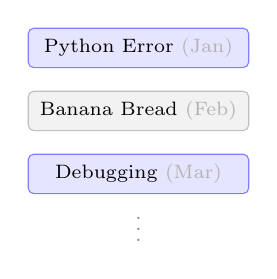
\begin{tikzpicture}
            % Simple list representation with topics
            \node[draw=blue!50, fill=blue!10, rounded corners=2pt,
                  minimum width=2.8cm, minimum height=0.5cm, font=\scriptsize]
                  (c1) at (0, 2.0) {Python Error \textcolor{gray!60}{(Jan)}};
            \node[draw=gray!50, fill=gray!10, rounded corners=2pt,
                  minimum width=2.8cm, minimum height=0.5cm, font=\scriptsize]
                  (c2) at (0, 1.2) {Banana Bread \textcolor{gray!60}{(Feb)}};
            \node[draw=blue!50, fill=blue!10, rounded corners=2pt,
                  minimum width=2.8cm, minimum height=0.5cm, font=\scriptsize]
                  (c3) at (0, 0.4) {Debugging \textcolor{gray!60}{(Mar)}};
            \node[font=\scriptsize, gray] at (0, -0.2) {$\vdots$};
        \end{tikzpicture}

        \vspace{0.2cm}
        {\scriptsize \textit{Just a timeline}}

        % --- MIDDLE: THE TRANSFORMATION ---
        \column{0.4\textwidth}
        \centering
        \textbf{\textcolor{blue!70}{The Transformation}}

        \vspace{0.3cm}

        
\begin{tikzpicture}
            \draw[->, ultra thick, blue!50] (0,0) -- (1.2,0);
        \end{tikzpicture}

        \vspace{0.3cm}

        \begin{block}{}
            \footnotesize
            \textbf{Nodes:} Each conversation $\rightarrow$ vector \textcolor{gray}{(embedding)}\\[0.15cm]
            \textbf{Edges:} Connect if similarity $> \theta$ \textcolor{gray}{(cosine)}\\
            {\scriptsize (similar direction $=$ similar meaning)}
        \end{block}

        % --- RIGHT: THE OUTPUT ---
        \column{0.3\textwidth}
        \centering
        \textbf{\textcolor{blue}{The Network}}

        \vspace{0.3cm}

        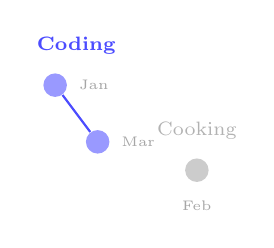
\begin{tikzpicture}[scale=0.9]
            % Coding cluster (connected) - Jan and Mar
            \node[circle, fill=blue!40, inner sep=3pt] (n1) at (0, 2.0) {};
            \node[font=\tiny, text=gray!70, anchor=west] at (0.2, 2.0) {Jan};
            \node[circle, fill=blue!40, inner sep=3pt] (n3) at (0.6, 1.2) {};
            \node[font=\tiny, text=gray!70, anchor=west] at (0.8, 1.2) {Mar};
            \draw[thick, blue!70] (n1) -- (n3);
            \node[font=\scriptsize, text=blue!70, anchor=south] at (0.3, 2.3) {\textbf{Coding}};

            % Banana bread (isolated)
            \node[circle, fill=gray!40, inner sep=3pt] (n2) at (2.0, 0.8) {};
            \node[font=\tiny, text=gray!70, anchor=north] at (2.0, 0.5) {Feb};
            \node[font=\scriptsize, text=gray!60, anchor=south] at (2.0, 1.1) {Cooking};
        \end{tikzpicture}

        \vspace{0.2cm}
        {\scriptsize \textit{Grouped by meaning}}
    \end{columns}

    \vspace{0.3cm}

    \begin{block}{The Key Insight}
        \centering
        \footnotesize
        Close in \textbf{time} $\neq$ close in \textbf{thought}.\\
        Jan and Mar snap together. Banana bread floats alone.
    \end{block}

    \note{
        \textbf{Slide 4: From Chat Logs to Network (1 min)}
        \begin{itemize}
            \item \textbf{Point LEFT (15s):} ``Here's your chat history. Just a list. One conversation after another, ordered by time.''
            \item \textbf{Point CENTER (25s):} ``Here's what we do. First, each conversation becomes a vector---an embedding. Then we measure similarity. Vectors pointing in similar directions mean similar topics. If similarity is above our threshold theta, we draw an edge.''
            \item \textbf{Point RIGHT (15s):} ``What comes out? A network grouped by meaning. Those two coding chats---January and March---they're connected now. Banana bread floats off on its own.''
            \item \textbf{Key Insight (5s):} ``Close in time doesn't mean close in thought. The network finds the real structure.''
        \end{itemize}
    }
\end{frame}

%---------------------------------------------------------
% 5. Pipeline: Intuition over Math
%---------------------------------------------------------
\begin{frame}{Whose Voice Matters?}
    \textbf{The Challenge:} AI responses are verbose and generic.\\
    \textbf{The Intuition:} User prompts carry the intent. But by how much?

    \vspace{0.2cm}

    \begin{columns}[T]
        \column{0.5\textwidth}
        \begin{block}{Separating Signal from Context}
            \begin{itemize}
                \item We separate \textbf{User Prompts} from \textbf{AI Replies}.
                \item \textbf{Weighting:} Introduce parameter $\alpha$ (user-to-AI ratio).
                \item \textbf{Question:} Does prioritizing the user actually improve structure?
            \end{itemize}
        \end{block}

        \vspace{0.2cm}
        {\tiny *Embeddings generated via nomic-embed-text (8k context).}

        \column{0.5\textwidth}
        \centering
        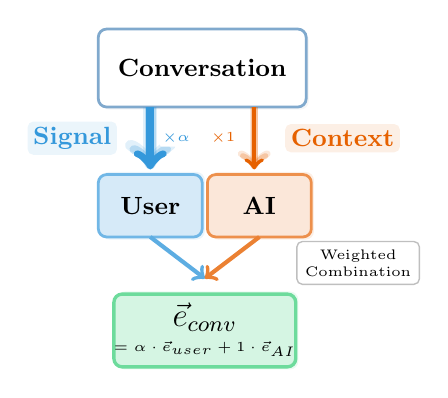
\begin{tikzpicture}[scale=0.66]
            % Conversation box with enhanced styling
            \fill[ShadowGray!15, rounded corners=3pt] (0.05,5.45) rectangle (4.05,6.95);
            \draw[rounded corners=3pt, thick, draw=PrimaryBlue!50, fill=white, line width=1pt]
                (0,5.5) rectangle (4,7);
            \node[align=center, font=\small\bfseries] at (2,6.25) {Conversation};

            % User arrow with glow effect
            \foreach \w/\op in {5pt/0.15, 4pt/0.25, 3pt/0.4} {
                \draw[->, line width=\w, TheoreticalBlue, opacity=\op] (1,5.5) -- (1,4.3);
            }
            \draw[->, line width=3pt, TheoreticalBlue] (1,5.5) -- (1,4.3);
            \node[TheoreticalBlue, font=\bfseries\small, fill=TheoreticalBlue!10,
                  rounded corners=2pt, inner sep=2pt] at (-0.5,4.9) {Signal};
            \node[TheoreticalBlue, font=\tiny\bfseries, fill=white,
                  rounded corners=1pt, inner sep=1pt] at (1.5,4.9) {$\times \alpha$};

            % AI arrow with subtle glow
            \foreach \w/\op in {3pt/0.15, 2.5pt/0.25} {
                \draw[->, line width=\w, AccentOrange, opacity=\op] (3,5.5) -- (3,4.3);
            }
            \draw[->, line width=1.5pt, AccentOrange] (3,5.5) -- (3,4.3);
            \node[AccentOrange, font=\bfseries\small, fill=AccentOrange!10,
                  rounded corners=2pt, inner sep=2pt] at (4.7,4.9) {Context};
            \node[AccentOrange, font=\tiny\bfseries, fill=white,
                  rounded corners=1pt, inner sep=1pt] at (2.4,4.9) {$\times 1$};

            % User box with shadow
            \fill[TheoreticalBlue!10, rounded corners=3pt] (0.05,2.95) rectangle (2.05,4.25);
            \draw[rounded corners=3pt, fill=TheoreticalBlue!20, draw=TheoreticalBlue!70, line width=1pt]
                (0,3) rectangle (2,4.2);
            \node[font=\small\bfseries] at (1,3.6) {User};

            % AI box with shadow
            \fill[AccentOrange!10, rounded corners=3pt] (2.15,2.95) rectangle (4.15,4.25);
            \draw[rounded corners=3pt, fill=AccentOrange!15, draw=AccentOrange!70, line width=1pt]
                (2.1,3) rectangle (4.1,4.2);
            \node[font=\small\bfseries] at (3.1,3.6) {AI};

            % Weighted combination arrows
            \draw[->, thick, TheoreticalBlue!80, line width=1.5pt] (1,3) -- (2.05,2.2);
            \draw[->, thick, AccentOrange!80, line width=1.5pt] (3.1,3) -- (2.05,2.2);

            % Weighted sum label in callout
            \node[font=\tiny, align=center, fill=white, rounded corners=2pt,
                  draw=gray!50, line width=0.5pt, inner sep=3pt] at (5.0,2.5) {Weighted\\Combination};

            % Final embedding with enhanced styling
            \fill[PracticalGreen!10, rounded corners=3pt] (0.35,0.45) rectangle (3.85,1.95);
            \draw[rounded corners=3pt, fill=PracticalGreen!20, draw=PracticalGreen!70, line width=1.2pt]
                (0.3,0.5) rectangle (3.8,1.9);
            \node[font=\large\bfseries] at (2.05,1.45) {$\vec{e}_{conv}$};
            \node[font=\tiny] at (2.05,0.85) {$= \alpha \cdot \vec{e}_{user} + 1 \cdot \vec{e}_{AI}$};
        \end{tikzpicture}
    \end{columns}

    \note{
        \textbf{Slide 5: Whose Voice Matters? (1 min)}
        \begin{itemize}
            \item \textbf{The Challenge (15s):} ``AI models are verbose. Full of boilerplate, helpful explanations, politeness. If you embed everything equally, the generic filler could drown out the actual signal---what you wanted to know.''
            \item \textbf{Point to Diagram - Top Split (20s):} [GESTURE TO FLOWCHART] ``So we split each conversation. User prompts on the left---intuitively, this is the \textbf{signal}, your intent. AI responses on the right---that's \textbf{context}.''
            \item \textbf{Point to Diagram - Weighting (15s):} ``We introduce a weighting parameter alpha. How much should we prioritize the user? Should we even prioritize the user at all?''
            \item \textbf{Point to Bottom - Final Embedding (10s):} [GESTURE TO BOTTOM] ``The result is this weighted conversation embedding. But what's the right alpha?''
            \item \textbf{Bridge (5s):} ``That's an empirical question. Let's test it.''
        \end{itemize}
    }
\end{frame}

%---------------------------------------------------------
% 6. Rigorous Parameter Tuning (2D Ablation Study)
%---------------------------------------------------------
\begin{frame}{Rigorous Parameter Tuning: 2D Ablation Study}
    \textbf{We ran a 63-configuration parameter sweep to maximize \textit{Modularity} (Q).}

    \vspace{0.3cm}

    \begin{columns}[T]
        % LEFT: Two plots stacked vertically
        \column{0.58\textwidth}

        % Top plot: Threshold evolution
        \centering
        \includegraphics[width=\textwidth, height=3.2cm, keepaspectratio]{images/threshold_evolution_clean.png}

        \vspace{0.3cm}

        % Bottom plot: Weight ratio
        \includegraphics[width=\textwidth, height=3.2cm, keepaspectratio]{images/weight_ratio_analysis_clean.png}

        % RIGHT: Unified findings
        \column{0.42\textwidth}
        \textbf{Two-Dimensional Sweep}

        \vspace{0.2cm}

        \begin{enumerate}
            \item \textbf{Threshold ($\theta$):}
            \begin{itemize}
                \scriptsize
                \item Phase transition at $\theta=0.875$
                \item \textbf{Choice: $\theta=0.9$} (optimizes modularity)
                \item Below: hairball; Above: fragmentation
            \end{itemize}

            \vspace{0.2cm}

            \item \textbf{Weight Ratio ($\alpha$):}
            \begin{itemize}
                \scriptsize
                \item \textbf{Confirmed:} Peak at $\alpha=2:1$
                \item User voice matters more $\rightarrow$ \textbf{Q = 0.750}
            \end{itemize}
        \end{enumerate}

        \vspace{0.2cm}
        {\scriptsize \textit{Data-driven validation of design choices.}}
    \end{columns}

    \note{
        \textbf{Slide 6: Rigorous Parameter Tuning (2 min)}
        \begin{itemize}
            \item \textbf{Opening - Set Context (30s):} ``We tested 63 configurations to answer two questions: what threshold theta? And does user weighting actually help?''
            \item \textbf{Point to TOP PLOT - Threshold Dimension (45s):} [GESTURE TO TOP PLOT] ``First: the similarity threshold. Look at this curve. Below 0.875, modularity crashes---everything connects into a hairball. We found a critical phase transition right at 0.875. We chose theta = 0.9---just past the transition. Data-driven, not guesswork.''
            \item \textbf{Point to BOTTOM PLOT - Weight Ratio (45s):} [GESTURE TO BOTTOM PLOT] ``Second: the weight ratio. Remember our intuition that user voice should matter more? The data confirms it. Modularity peaks precisely at 2:1. Not 1:1, not 3:1. The user's intent really does drive the structure. Q = 0.750.''
            \item \textbf{Conclusion (10s):} ``The ablation study serves two purposes: it confirms our intuition, and it finds the optimal ratio. These choices aren't arbitrary.''
        \end{itemize}
    }
\end{frame}

%---------------------------------------------------------
% 8. The Cognitive MRI: Network Visualization
%---------------------------------------------------------
\begin{frame}{The Cognitive MRI: 15 Knowledge Domains}
    \centering
    \includegraphics[width=\textwidth, height=0.85\textheight, keepaspectratio]{cluster-vis-topics-better.png}

    \note{
        \textbf{Slide 7: The Reveal (1.5 min)}
        \begin{itemize}
            \item \textbf{PAUSE FOR EFFECT (5s):} [ADVANCE SLIDE, LET IMAGE FILL SCREEN, SILENCE] \textit{Let them absorb the network.}
            \item \textbf{The Numbers (15s):} ``Hundreds of nodes, thousands of edges. Modularity 0.75. 15 communities---15 knowledge domains.''
            \item \textbf{Labeling (15s):} ``I labeled these communities manually by inspecting each one. Though I did try having an LLM automate it, and it worked reasonably well.''
            \item \textbf{Walk Through Communities (45s):} [GESTURE TO CLUSTERS] ``Let me walk you through the major domains. Up here, my master's thesis work in pure math. Next to it, stats and probability. Over here, ML and AI. Philosophy and alignment. Down here, coding projects---more spread out, different projects in their own clusters.''
            \item \textbf{Key Point (10s):} ``The communities were \textit{discovered} by the algorithm. I just interpreted what they mean.''
        \end{itemize}
    }
\end{frame}

%---------------------------------------------------------
% 9. Insight 1: Structural Heterogeneity
%---------------------------------------------------------
\begin{frame}{Insight 1: Structural Heterogeneity}
    \centering
    \textbf{Knowledge isn't uniform. Theoretical and practical thinking have distinct shapes.}

    \vspace{0.15cm}

    \begin{columns}[T]
        % --- LEFT COLUMN: THEORETICAL (Small World) ---
        \column{0.48\textwidth}
        \centering
        \textbf{\textcolor{TheoreticalBlue}{Theoretical Domains}} \\
        \scriptsize \textit{(Math, Philosophy, ML Theory)}

        \vspace{0.1cm}
        % Enhanced Small World / Mesh with depth
        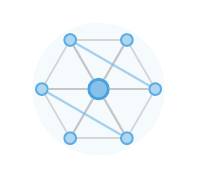
\begin{tikzpicture}[scale=0.6, baseline=(current bounding box.center)]
            \path[use as bounding box] (-1.5,-1.3) rectangle (1.5,1.3);

            % Background glow for cluster
            \fill[TheoreticalBlue!10, opacity=0.5] (0,0) circle (1.4cm);

            % Central hub with glow
            \fill[TheoreticalBlue!50, opacity=0.4] (0,0) circle (0.15cm);
            \node[circle, fill=TheoreticalBlue!60, draw=TheoreticalBlue!90,
                  line width=1pt, inner sep=2.5pt] (c) at (0,0) {};

            % Peripheral nodes with glow
            \foreach \i in {0,60,...,300} {
                \fill[TheoreticalBlue!30, opacity=0.3] (\i:1.2) circle (0.12cm);
                \node[circle, fill=TheoreticalBlue!40, draw=TheoreticalBlue!80,
                      line width=0.7pt, inner sep=1.5pt] (n\i) at (\i:1.2) {};
            }

            % Connections with depth
            \foreach \i in {0,60,...,300} {
                \draw[gray!60, line width=0.8pt, opacity=0.7] (c) -- (n\i);
                \pgfmathsetmacro{\nextangle}{int(mod(\i+60,360))}
                \draw[gray!60, line width=0.6pt, opacity=0.5] (n\i) -- (n\nextangle);
            }
            % Cross-connections for small-world
            \draw[TheoreticalBlue!70, line width=0.8pt, opacity=0.6] (n0) -- (n120);
            \draw[TheoreticalBlue!70, line width=0.8pt, opacity=0.6] (n180) -- (n300);
        \end{tikzpicture}

        \vspace{0.1cm}
        \begin{block}{``Small-World'' Structures}
            \footnotesize
            \begin{itemize}
                \item \textbf{Dense Clustering ($C \approx 0.58$):} Concepts are highly interconnected.
                \item \textbf{Recursive:} Frequent backtracking to refine core definitions (e.g., axioms, ethics).
            \end{itemize}
        \end{block}

        % --- RIGHT COLUMN: PRACTICAL (Tree-Like) ---
        \column{0.48\textwidth}
        \centering
        \textbf{\textcolor{green!40!black}{Practical Domains}} \\
        \scriptsize \textit{(Programming Projects, Debugging)}

        \vspace{0.1cm}
        % Enhanced Tree Structure with depth effects
        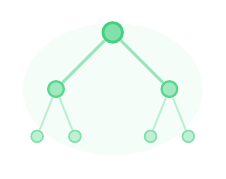
\begin{tikzpicture}[scale=0.6, baseline=(current bounding box.center)]
            % Invisible bounding box for consistent height
            \path[use as bounding box] (-1.8,-1.3) rectangle (1.8,1.3);

            % Subtle background gradient for tree region
            \fill[PracticalGreen!8, opacity=0.6] (0,0) ellipse (1.9cm and 1.4cm);

            % Root node with glow
            \fill[PracticalGreen!40, opacity=0.4] (0,1.2) circle (0.15cm);
            \node[circle, fill=PracticalGreen!60, draw=PracticalGreen!90,
                  line width=1pt, inner sep=2.5pt] (root) at (0,1.2) {};

            % Level 1 nodes with glow
            \fill[PracticalGreen!30, opacity=0.3] (-1.2,0) circle (0.12cm);
            \node[circle, fill=PracticalGreen!45, draw=PracticalGreen!80,
                  line width=0.8pt, inner sep=2pt] (l1) at (-1.2, 0) {};
            \fill[PracticalGreen!30, opacity=0.3] (1.2,0) circle (0.12cm);
            \node[circle, fill=PracticalGreen!45, draw=PracticalGreen!80,
                  line width=0.8pt, inner sep=2pt] (r1) at (1.2, 0) {};

            % Level 2 nodes (leaves) with subtle glow
            \foreach \x/\y in {-1.6/-1, -0.8/-1, 0.8/-1, 1.6/-1} {
                \fill[PracticalGreen!20, opacity=0.25] (\x,\y) circle (0.1cm);
            }
            \node[circle, fill=PracticalGreen!30, draw=PracticalGreen!60,
                  line width=0.6pt, inner sep=1.5pt] (l2a) at (-1.6, -1) {};
            \node[circle, fill=PracticalGreen!30, draw=PracticalGreen!60,
                  line width=0.6pt, inner sep=1.5pt] (l2b) at (-0.8, -1) {};
            \node[circle, fill=PracticalGreen!30, draw=PracticalGreen!60,
                  line width=0.6pt, inner sep=1.5pt] (r2a) at (0.8, -1) {};
            \node[circle, fill=PracticalGreen!30, draw=PracticalGreen!60,
                  line width=0.6pt, inner sep=1.5pt] (r2b) at (1.6, -1) {};

            % Enhanced connections with depth - thicker near root
            \draw[PracticalGreen!60, line width=1pt, opacity=0.8] (root) -- (l1);
            \draw[PracticalGreen!60, line width=1pt, opacity=0.8] (root) -- (r1);
            \draw[PracticalGreen!50, line width=0.7pt, opacity=0.6] (l1) -- (l2a);
            \draw[PracticalGreen!50, line width=0.7pt, opacity=0.6] (l1) -- (l2b);
            \draw[PracticalGreen!50, line width=0.7pt, opacity=0.6] (r1) -- (r2a);
            \draw[PracticalGreen!50, line width=0.7pt, opacity=0.6] (r1) -- (r2b);
        \end{tikzpicture}

        \vspace{0.1cm}
        \begin{block}{Tree-Like Expansion}
            \footnotesize
            \begin{itemize}
                \item \textbf{Branching ($C \approx 0.39$):} Task-based exploration without backtracking.
                \item \textbf{Independent:} Projects form isolated silos (e.g., \emph{Metaprogramming} vs. \emph{Physics Sim}).
            \end{itemize}
        \end{block}
    \end{columns}

    \note{
        \textbf{Slide 8: Insight 1 - Heterogeneity (1.5 min)}
        \begin{itemize}
            \item \textbf{Opening - The Big Idea (15s):} ``Here's the first major finding: not all knowledge looks the same. Different domains have fundamentally different \textit{shapes}.''
            \item \textbf{Point to Table - Metrics (20s):} [GESTURE TO TABLE] ``Look at these numbers. Theoretical domains: clustering coefficient 0.58. Practical domains: 0.39. That's a massive difference. Path length also differs---2.3 versus 3.1.''
            \item \textbf{Point to LEFT - Theory Diagram (30s):} [GESTURE TO LEFT DIAGRAM] ``Theoretical topics---math, philosophy, ML theory---are `Small-World' structures. Look at this dense mesh. High clustering. Why? You define a concept, you reuse it across many conversations, you refine it. Recursive thinking. Lots of backtracking and cross-references.''
            \item \textbf{Point to RIGHT - Practice Diagram (30s):} [GESTURE TO RIGHT DIAGRAM] ``Practical coding? Tree-like. Lower clustering. You solve Bug A, move to Bug B. Branching, forward exploration. Projects are isolated---my physics sim doesn't talk to my web dev project. Different cognitive patterns entirely.''
            \item \textbf{Significance (15s):} ``This structural heterogeneity---this within-network diversity---is unique to conversation networks. You don't see this in homogeneous citation networks.''
        \end{itemize}
    }
\end{frame}

%---------------------------------------------------------
% 10. Insight 2: A Taxonomy of Bridges
%---------------------------------------------------------
\begin{frame}{Insight 2: A Taxonomy of Bridges}
    \begin{columns}[T]
        \column{0.55\textwidth}
        \centering
        \includegraphics[width=\textwidth, height=0.8\textheight, keepaspectratio]{images/bridge-better.png}

        \column{0.45\textwidth}
        \textit{The network reveals three distinct bridging mechanisms.}
        \vspace{0.2cm}

        \textcolor{blue}{\textbf{1. Evolutionary Bridges}} \\
        { \scriptsize
        \textit{(e.g., Geometric Mean)}\\
        Conversations that \textbf{drift}: \textcolor{purple!70!black}{Stats} $\rightarrow$ \textcolor{green!60!black}{ML/AI} $\rightarrow$ \textcolor{orange!80!black}{Programming}.
        }
        \vspace{0.2cm}

        \textcolor{teal}{\textbf{2. Integrative Bridges}} \\
        { \scriptsize
        \textit{(e.g., mcts-code)}\\
        Deliberate synthesis: \textcolor{green!60!black}{AI/ML} $\leftrightarrow$ \textcolor{orange!80!black}{Programming}.
        }
        \vspace{0.2cm}

        \textcolor{orange!80!black}{\textbf{3. Pure Bridges}} \\
        { \scriptsize
        \textit{(e.g., cuda-program-linux)}\\
        \textbf{Rare shortcuts:} \textcolor{red!70!black}{Physics Sim} $\leftrightarrow$ \textcolor{blue!70!black}{Programming}.
        }
    \end{columns}

    \note{
        \textbf{Slide 9: Insight 2 - Bridge Taxonomy (1.5 min)}
        \begin{itemize}
            \item \textbf{Opening Question (15s):} ``Second finding: How do ideas move between these isolated knowledge islands? The network reveals three distinct bridging mechanisms.''
            \item \textbf{Point to Visualization (15s):} [GESTURE TO LEFT IMAGE] ``This visualization shows high-betweenness nodes---the bridges. Notice they're not all the same type.''
            \item \textbf{Type 1 - Evolutionary (30s):} ``First: Evolutionary Bridges. Conversations that \textit{drift}. The `Geometric Mean' conversation started in statistics and probability, drifted through ML and AI concepts, ended up in practical programming. Natural topic evolution. You didn't plan to cross domains---it just happened through the flow of ideas.''
            \item \textbf{Type 2 - Integrative (30s):} ``Second: Integrative Bridges. Deliberate synthesis. `mcts-code'---Monte Carlo Tree Search implementation---explicitly combines AI and ML concepts with practical programming. You're consciously building connections between theory and practice.''
            \item \textbf{Type 3 - Pure Bridges (20s):} ``Third: Pure Bridges---rare shortcuts. A single conversation connecting otherwise distant clusters. `cuda-program-linux'---a Linux config question that happens to link my physics simulation work with practical programming. Rare, but powerful.''
            \item \textbf{Bridge (5s):} ``These bridges---these connections across domains---are precisely what makes the map useful. Here's why...''
        \end{itemize}
    }
\end{frame}

%---------------------------------------------------------
% 11. The Vision: Personal Knowledge Cartography
%---------------------------------------------------------
\begin{frame}{The Vision: Personal Knowledge Cartography}
    \centering
    \textbf{Why do we need this map?}

    \vspace{0.05cm}

    % The Graphic: Reduced scale to 0.7 to fit slide
    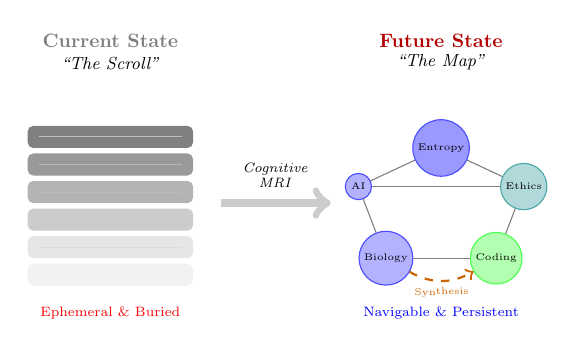
\begin{tikzpicture}[scale=0.7, transform shape]
        % --- LEFT SIDE: THE SCROLL (Current State) ---
        \node[anchor=south] at (1.5, 4.2) {\textbf{\textcolor{gray}{Current State}}};
        \node[anchor=south] at (1.5, 3.8) {\small \textit{``The Scroll''}};

        % Draw a stack of fading bars
        \foreach \y/\opacity in {0/0.1, 0.5/0.2, 1.0/0.4, 1.5/0.6, 2.0/0.8, 2.5/1.0} {
            \draw[fill=gray, opacity=\opacity, draw=none, rounded corners=2pt]
                (0, \y) rectangle (3, \y+0.4);
            \draw[gray!50, opacity=\opacity] (0.2, \y+0.2) -- (2.8, \y+0.2);
        }

        % Label for the problem
        \node[align=center, font=\scriptsize, text=red] at (1.5, -0.5)
            {Ephemeral \& Buried};

        % --- ARROW: THE TRANSFORMATION ---
        \draw[->, line width=1mm, gray!40] (3.5, 1.5) -- (5.5, 1.5);
        \node[font=\scriptsize, align=center] at (4.5, 2) {\textit{Cognitive}\\ \textit{MRI}};

        % --- RIGHT SIDE: THE MAP (Future State) ---
        \node[anchor=south] at (7.5, 4.2) {\textbf{\textcolor{red!70!black}{Future State}}};
        \node[anchor=south] at (7.5, 3.8) {\small \textit{``The Map''}};

        % Define nodes (colors match cluster-vis theoretical/practical palette)
        \node[circle, fill=blue!30, draw=blue!70, inner sep=2pt, font=\tiny] (bio) at (6.5, 0.5) {Biology};
        \node[circle, fill=green!30, draw=green!70, inner sep=2pt, font=\tiny] (code) at (8.5, 0.5) {Coding};
        \node[circle, fill=blue!40, draw=blue!70, inner sep=2pt, font=\tiny] (entropy) at (7.5, 2.5) {Entropy};
        \node[circle, fill=blue!30, draw=blue!70, inner sep=2pt, font=\tiny] (ai) at (6, 1.8) {AI};
        \node[circle, fill=teal!30, draw=teal!70, inner sep=2pt, font=\tiny] (ethics) at (9, 1.8) {Ethics};

        % Draw connections
        \draw[gray] (bio) -- (ai);
        \draw[gray] (ai) -- (entropy);
        \draw[gray] (entropy) -- (ethics);
        \draw[gray] (ethics) -- (code);
        \draw[gray] (bio) -- (code);
        \draw[gray] (ai) -- (ethics);

        % Highlight the "Synthesis" path
        \draw[orange!80!black, thick, dashed, ->] (bio) to[bend right=30]
            node[midway, below, sloped, font=\tiny, text=orange!80!black] {Synthesis} (code);

        % Label for the solution
        \node[align=center, font=\scriptsize, text=blue] at (7.5, -0.5)
            {Navigable \& Persistent};
    \end{tikzpicture}

    \vspace{0.1cm}

    % Concrete example box
    \begin{tcolorbox}[colback=blue!5, colframe=blue!40, boxrule=0.5pt, arc=2pt, left=3pt, right=3pt, top=2pt, bottom=2pt]
        \scriptsize
        \textbf{Example Query:} \textit{``Show me everywhere I discussed entropy.''} \\
        \textbf{Result:} Network lights up connections: Biology $\leftrightarrow$ AI Theory $\leftrightarrow$ Coding $\leftrightarrow$ Ethics
    \end{tcolorbox}

    \vspace{0.05cm}

    % Simplified text - just the core contrast
    \begin{columns}[T]
        \column{0.5\textwidth}
        \centering
        \scriptsize
        \textbf{Problem:} Insights buried \\in infinite scroll

        \column{0.5\textwidth}
        \centering
        \scriptsize
        \textbf{Solution:} Navigate \& synthesize \\across your entire history
    \end{columns}

    \note{
        \textbf{Slide 10: Vision (30s MAX - don't linger)}
        \begin{itemize}
            \item \textbf{Quick Contrast (15s):} ``Why does this matter? Right now, your chat history is an infinite scroll. Buried. The map makes it navigable.''
            \item \textbf{One Example (15s):} ``Imagine: `Show me everywhere I discussed entropy.' The network lights up---connections you forgot about.''
            \item \textbf{Move On:} Don't elaborate. The visual speaks. Go to conclusion.
        \end{itemize}
    }
\end{frame}

%---------------------------------------------------------
% 12. Conclusion & Impact
%---------------------------------------------------------
\begin{frame}[fragile]{Cognitive MRI: A Proof of Concept}
    \begin{columns}[T]
        % COLUMN 1: FINDINGS
        \column{0.31\textwidth}
        \begin{exampleblock}{Key Findings}
            \centering
            \includegraphics[width=0.5\textwidth]{images/cluster-vis-topics-better.png}
            \vspace{0.02cm}
            \begin{itemize}
                \scriptsize
                \item \textbf{Method:} Tuned user-weighting (2:1) and link thresholds (for modularity).
                \item \textbf{Topology:} Heterogeneous (Hubs vs. Trees).
                \item \textbf{Bridges:} Evolutionary, Integrative, \& Pure.
            \end{itemize}
        \end{exampleblock}

        \hspace{0.01\textwidth}

        % COLUMN 2: LIMITATIONS
        \column{0.31\textwidth}
        \begin{alertblock}{Limitations}
            \centering
            \vspace{0.02cm}
            % Enhanced TikZ: Single user with snapshot camera
            \begin{tikzpicture}[scale=0.9]
                % Subtle background glow
                \fill[AccentOrange!8, opacity=0.5] (0,0) circle (0.85cm);
                % Main user circle with glow effect
                \fill[AccentOrange!25, opacity=0.4] (0,0) circle (0.72cm);
                \node[circle, fill=AccentOrange!20, draw=AccentOrange!60, line width=1.2pt, inner sep=16pt] (user) at (0,0) {};
                \node[font=\Large, text=AccentOrange!80!black] at (0,0.15) {\faUser};
                \node[font=\scriptsize\bfseries, text=AccentOrange!80!black] at (0,-0.5) {N=1};
                % Camera icon with subtle glow
                \fill[gray!15, opacity=0.4] (1.5,1.0) circle (0.25cm);
                \node[font=\small, text=gray!70] at (1.5,1.0) {\faCamera};
            \end{tikzpicture}
            \vspace{0.02cm}
            \begin{itemize}
                \scriptsize
                \item Single User \& Platform.
                \item Snapshot in time.
                \item Exploratory (No ``Ground Truth'').
            \end{itemize}
        \end{alertblock}

        \hspace{0.01\textwidth}

        % COLUMN 3: FUTURE
        \column{0.31\textwidth}
        \begin{block}{Future Directions}
            \centering
            \vspace{0.02cm}
            % Enhanced TikZ: Growth from 1 to many with temporal evolution + validation
            \begin{tikzpicture}[scale=0.85]
                % Single node on left with glow
                \fill[TheoreticalBlue!20, opacity=0.4] (0,0) circle (0.18cm);
                \node[circle, fill=TheoreticalBlue!40, draw=TheoreticalBlue!70, line width=1pt, inner sep=3pt] (one) at (0,0) {};
                % Enhanced arrow with glow
                \foreach \w/\op in {4pt/0.15, 3pt/0.25} {
                    \draw[->, line width=\w, PrimaryBlue!40, opacity=\op] (0.4,0) -- (2.2,0);
                }
                \draw[->, line width=2pt, PrimaryBlue!50] (0.4,0) -- (2.2,0);
                \node[font=\tiny\bfseries, text=PrimaryBlue!70, above, fill=white, inner sep=1pt, rounded corners=1pt] at (1.3,0.15) {scale + time};
                % Background glow for network cluster
                \fill[PracticalGreen!10, opacity=0.5] (3.2,0) circle (1.1cm);
                % Multiple nodes on right with glows - varying sizes for diversity
                \foreach \x/\y in {2.8/0.7, 3.2/0, 2.8/-0.7, 3.7/0.4, 3.7/-0.4} {
                    \fill[PracticalGreen!25, opacity=0.3] (\x,\y) circle (0.12cm);
                }
                \node[circle, fill=PracticalGreen!50, draw=PracticalGreen!80, line width=0.8pt, inner sep=4pt] (n1) at (2.8, 0.7) {};
                \node[circle, fill=PracticalGreen!40, draw=PracticalGreen!70, line width=0.8pt, inner sep=3pt] (n2) at (3.2, 0) {};
                \node[circle, fill=PracticalGreen!50, draw=PracticalGreen!80, line width=0.8pt, inner sep=3.5pt] (n3) at (2.8, -0.7) {};
                \node[circle, fill=PracticalGreen!30, draw=PracticalGreen!60, line width=0.6pt, inner sep=2.5pt] (n4) at (3.7, 0.4) {};
                \node[circle, fill=PracticalGreen!45, draw=PracticalGreen!75, line width=0.7pt, inner sep=3pt] (n5) at (3.7, -0.4) {};
                % Connection lines with depth
                \draw[PracticalGreen!50, line width=0.8pt, opacity=0.7] (n1) -- (n2) -- (n3);
                \draw[PracticalGreen!40, line width=0.6pt, opacity=0.5] (n2) -- (n4);
                \draw[PracticalGreen!40, line width=0.6pt, opacity=0.5] (n2) -- (n5);
                % Validation: magnifying glass with subtle glow
                \fill[TheoreticalBlue!15, opacity=0.4] (4.3, 0) circle (0.25cm);
                \node[font=\normalsize, text=TheoreticalBlue!70] at (4.3, 0) {\faSearch};
            \end{tikzpicture}
            \vspace{0.02cm}
            \begin{itemize}
                \scriptsize
                \item \textbf{Scale:} More users \& cross-platform analysis.
                \item \textbf{Longitudinal:} Track knowledge evolution over time.
                \item \textbf{Validation:} User studies.
            \end{itemize}
        \end{block}
    \end{columns}

    \vspace{0cm}
    \centering
    \tiny \faGithub\ \texttt{github.com/queelius/chatgpt-complex-net}
\end{frame}

% NOTE: Placed OUTSIDE frame because [fragile] frames cannot contain \note
\note{
    \textbf{Slide 11: Conclusion - Proof of Concept (1 min)}
    \begin{itemize}
        \item \textbf{Opening Summary (20s):} ``We've demonstrated a proof of concept: LLM conversation logs can be transformed into meaningful cognitive maps showing the latent structure of knowledge.''
        \item \textbf{Point to LEFT - Key Findings (20s):} [GESTURE TO NETWORK IMAGE] ``User-weighted embeddings to capture intent. Heterogeneous topology---theoretical domains look fundamentally different from practical ones. A taxonomy of three bridge types. All validated through rigorous 2D ablation studies.''
        \item \textbf{Point to MIDDLE - Acknowledge Limits (10s):} [GESTURE TO N=1 ICON] ``This is N=1. A single user, single platform, snapshot in time. No ground truth validation yet.''
        \item \textbf{Point to RIGHT - The Path Forward (10s):} [GESTURE TO GROWTH DIAGRAM] ``But those limitations point the way forward. Scale to cohorts. Track longitudinal evolution. Validate with user studies.''
        \item \textbf{Closing (5s):} ``Thank you. Happy to take questions.''
    \end{itemize}
}

%---------------------------------------------------------
% BACKUP SLIDE: Technical Details (for Q&A only)
%---------------------------------------------------------
\begin{frame}[noframenumbering]{Backup: Technical Details}
    \textbf{Embedding Details}
    \begin{itemize}
        \scriptsize
        \item Model: \texttt{nomic-embed-text} (8k context window)
        \item Dimension: 768
        \item Chunking: 500-token windows with 50-token overlap
        \item User-to-AI weighting: 2:1 ratio (validated via ablation study)
    \end{itemize}

    \vspace{0.3cm}

    \textbf{Community Detection}
    \begin{itemize}
        \scriptsize
        \item Algorithm: Louvain (resolution = 1.0)
        \item Modularity: Q = 0.750 (15 communities discovered)
        \item Giant component: $\sim$500 nodes, $\sim$1,600 edges
    \end{itemize}

    \vspace{0.3cm}

    \textbf{Dataset Filtering}
    \begin{itemize}
        \scriptsize
        \item Original dataset: 1,908 conversations (2--3 years)
        \item After similarity threshold ($\theta=0.9$): $\sim$500 conversations in giant component
        \item Isolated nodes filtered: conversations with no semantic neighbors
    \end{itemize}

    \vspace{0.3cm}

    \centering
    \footnotesize
    \textbf{Full methodology \& code:} \faGithub\ \texttt{github.com/queelius/chatgpt-complex-net}
\end{frame}

%---------------------------------------------------------
% BACKUP SLIDE 2: Core Formulas (for Q&A only)
%---------------------------------------------------------
\begin{frame}[noframenumbering]{Backup: Core Formulas}

    \begin{columns}[T]
        \column{0.5\textwidth}
        \small

        \textbf{Weighted Embedding}
        \vspace{-0.1cm}
        \begin{equation*}
            \footnotesize
            \vec{e}_{conv} = \frac{\alpha \vec{e}_{user} + \vec{e}_{AI}}{\|\alpha \vec{e}_{user} + \vec{e}_{AI}\|}
        \end{equation*}
        \vspace{-0.15cm}
        {\scriptsize $\alpha = 2$ (2:1 weighting)}

        \vspace{0.3cm}

        \textbf{Modularity (Newman's Q)}
        \vspace{-0.1cm}
        \begin{equation*}
            \footnotesize
            Q = \frac{1}{2m} \sum_{ij} \left[ A_{ij} - \frac{k_i k_j}{2m} \right] \delta(c_i, c_j)
        \end{equation*}
        \vspace{-0.15cm}
        {\scriptsize $A_{ij}$: adjacency, $k_i$: degree, $m$: edges}

        \column{0.5\textwidth}
        \small

        \textbf{Betweenness Centrality}
        \vspace{-0.1cm}
        \begin{equation*}
            \footnotesize
            B(v) = \sum_{s \neq v \neq t} \frac{\sigma_{st}(v)}{\sigma_{st}}
        \end{equation*}
        \vspace{-0.15cm}
        {\scriptsize $\sigma_{st}$: shortest paths $s \to t$}

        \vspace{0.3cm}

        \textbf{Clustering Coefficient}
        \vspace{-0.1cm}
        \begin{equation*}
            \footnotesize
            C_i = \frac{2e_i}{k_i(k_i - 1)}
        \end{equation*}
        \vspace{-0.15cm}
        {\scriptsize $e_i$: edges among neighbors}
    \end{columns}

\end{frame}

%---------------------------------------------------------
% BACKUP SLIDE 3: Privacy & Data Handling (for Q&A only)
%---------------------------------------------------------
\begin{frame}[noframenumbering]{Backup: Privacy \& Data Handling}
    \begin{columns}[T]
        \column{0.5\textwidth}
        \textbf{This Study}
        \begin{itemize}
            \scriptsize
            \item \textbf{Consent:} Author's own conversations
            \item \textbf{Export:} Official ChatGPT data export
            \item \textbf{Content:} Exploratory/academic only
            \item \textbf{Sharing:} Aggregated statistics, no raw logs
        \end{itemize}

        \vspace{0.2cm}

        \textbf{Code Release}
        \begin{itemize}
            \scriptsize
            \item Framework is open-source
            \item Users run locally on their own data
            \item No data leaves user's machine
        \end{itemize}

        \column{0.5\textwidth}
        \textbf{Future Multi-User Studies}
        \begin{itemize}
            \scriptsize
            \item \textbf{IRB Required:} Formal ethics review
            \item \textbf{Informed Consent:} Explicit opt-in
            \item \textbf{Anonymization:}
                \begin{itemize}
                    \tiny
                    \item Remove PII (names, emails)
                    \item Hash conversation IDs
                    \item Redact sensitive topics
                \end{itemize}
            \item \textbf{Differential Privacy:} For aggregate statistics
        \end{itemize}

        \vspace{0.2cm}

        \begin{alertblock}{\scriptsize Key Principle}
            \tiny
            Designed for \textbf{self-knowledge}---users mapping their own thought, not surveillance.
        \end{alertblock}
    \end{columns}
\end{frame}

%---------------------------------------------------------
% BACKUP SLIDE 4: Methodology Alternatives (for Q&A only)
%---------------------------------------------------------
\begin{frame}[noframenumbering]{Backup: Methodology Alternatives}
    \textbf{Why These Design Choices?}

    \vspace{0.1cm}

    \scriptsize
    \begin{tabular}{@{}p{2.2cm}p{2.5cm}p{5cm}@{}}
        \toprule
        \textbf{Choice} & \textbf{Alternative} & \textbf{Why We Chose This} \\
        \midrule
        \textbf{Cosine Similarity} & Euclidean Distance & Magnitude-invariant (length $\neq$ relevance) \\
        & Jaccard (set-based) & Semantic continuity, not just keywords \\
        \midrule
        \textbf{Threshold} ($\theta$=0.9) & Soft/fuzzy clustering & Clear community boundaries \\
        & k-NN graph & Ablation validated hard threshold \\
        \midrule
        \textbf{nomic-embed-text} & OpenAI embeddings & Open weights, 8k context, reproducible \\
        & Sentence-BERT & Better long-context handling \\
        \midrule
        \textbf{2:1 Weighting} & Equal (1:1) & AI responses dilute user intent \\
        & User-only & Loses conversational context \\
        \bottomrule
    \end{tabular}

    \vspace{0.2cm}

    \centering
    \tiny
    \textit{All choices validated via 63-configuration ablation study (Slide 6)}
\end{frame}

\end{document}
